

\tikzset{every picture/.style={line width=0.75pt}} %set default line width to 0.75pt

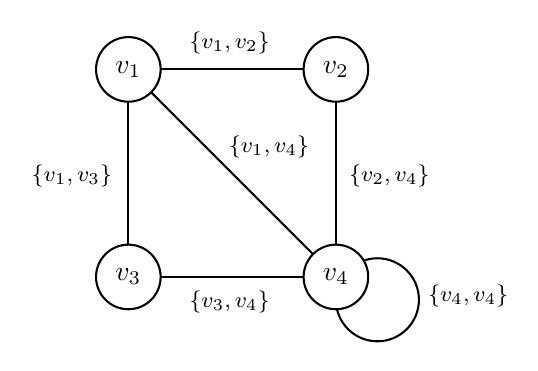
\begin{tikzpicture}[x=0.75pt,y=0.75pt,yscale=-1,xscale=1]
%uncomment if require: \path (0,178); %set diagram left start at 0, and has height of 178

%Shape: Circle [id:dp5100735212019099]
\draw   (430,141) .. controls (430,129.95) and (438.95,121) .. (450,121) .. controls (461.05,121) and (470,129.95) .. (470,141) .. controls (470,152.05) and (461.05,161) .. (450,161) .. controls (438.95,161) and (430,152.05) .. (430,141) -- cycle ;

% Text Node
\draw (473,132.4) node [anchor=north west][inner sep=0.75pt]  [font=\footnotesize]  {$\{v_{4} ,v_{4}\}$};
% Text Node
\draw (358,135.4) node [anchor=north west][inner sep=0.75pt]  [font=\footnotesize]  {$\{v_{3} ,v_{4}\}$};
% Text Node
\draw    (330, 30) circle [x radius= 15.56, y radius= 15.56]   ;
\draw (330,30) node   [align=left] {\begin{minipage}[lt]{13.600000000000001pt}\setlength\topsep{0pt}
\begin{center}
$\displaystyle v_{1}$
\end{center}

\end{minipage}};
% Text Node
\draw    (330, 130) circle [x radius= 15.56, y radius= 15.56]   ;
\draw (330,130) node   [align=left] {\begin{minipage}[lt]{13.600000000000001pt}\setlength\topsep{0pt}
\begin{center}
$\displaystyle v_{3}$
\end{center}

\end{minipage}};
% Text Node
\draw  [fill={rgb, 255:red, 255; green, 255; blue, 255 }  ,fill opacity=1 ]  (430, 130) circle [x radius= 15.56, y radius= 15.56]   ;
\draw (430,130) node   [align=left] {\begin{minipage}[lt]{13.600000000000001pt}\setlength\topsep{0pt}
\begin{center}
$\displaystyle v_{4}$
\end{center}

\end{minipage}};
% Text Node
\draw    (430, 30) circle [x radius= 15.56, y radius= 15.56]   ;
\draw (430,30) node   [align=left] {\begin{minipage}[lt]{13.600000000000001pt}\setlength\topsep{0pt}
\begin{center}
$\displaystyle v_{2}$
\end{center}

\end{minipage}};
% Text Node
\draw (358,10.4) node [anchor=north west][inner sep=0.75pt]  [font=\footnotesize]  {$\{v_{1} ,v_{2}\}$};
% Text Node
\draw (377,60.4) node [anchor=north west][inner sep=0.75pt]  [font=\footnotesize]  {$\{v_{1} ,v_{4}\}$};
% Text Node
\draw (435,74.4) node [anchor=north west][inner sep=0.75pt]  [font=\footnotesize]  {$\{v_{2} ,v_{4}\}$};
% Text Node
\draw (282,74.4) node [anchor=north west][inner sep=0.75pt]  [font=\footnotesize]  {$\{v_{1} ,v_{3}\}$};
% Connection
\draw    (341,41) -- (419,119) ;
% Connection
\draw    (345.56,30) -- (414.44,30) ;
% Connection
\draw    (430,45.56) -- (430,114.44) ;
% Connection
\draw    (345.56,130) -- (414.44,130) ;
% Connection
\draw    (330,45.56) -- (330,114.44) ;

\end{tikzpicture}